% 学位论文 : 第三章 GaAs/Si异变外延两步法生长
% 
% 更新记录:
%   {$LastChangedBy$}
%   {$LastChangedRevision$}
%   {$LastChangedDate$}

\chapter{GaAs/Si异变外延两步法生长}

\section{GaAs/Si异变外延两步法生长,问题,目标}

GaAs与Si之间\%4的晶格失配对于在Si衬底上生长高质量GaAs外延片是最大的阻碍,Si衬底上最初的GaAs成核是生长过程中的关键步骤,并且在一定程度上决定着上面GaAs的质量。

晶片生长的成核有三种生长模式:层状生长(FM),岛状生长(VM)和SK模式生长,其中SK模式生长即是先岛状生长,接着是浸润层状生长。
前两种生长模式(FM和VM)可以用衬底表面能($ \gamma_{s}$)、外延层表面能($\gamma_{f}$)和两者之间的界面能($\gamma_{i}$)之间的关系来区分,如果衬底表面能远大于其他两者之和,则浸润机制发生,即是FM生长机制:

\begin{equation}
	\label{eq:FM}
 	\gamma_{s} > \gamma_{f} + \gamma_{i}
\end{equation}

若相反

\begin{equation}
	\label{eq:VM}
 	\gamma_{s} < \gamma_{f} + \gamma_{i}
\end{equation}

则无浸润发生,也就是VM生长机制。

对于SK生长模式,在开始生长阶段,表面能之间的关系是\ref{eq:FM},而在生长几个原子层之后表面能之间的关系则转换为\ref{eq:VM}。

GaAs/Si外延生长不包括浸润层,GaAs岛直接在Si衬底上形成,因此GaAs/Si最初的生长机制是VM。
Adomi 等阐述了衬底表面能的减少在GaAs/Si生长的过程中所起到的重要作用。他们在GaAs衬底上生长了0.9nm的Si薄膜(Si是赝形生长),然后再外延GaAs,则GaAs最初是岛状生长。以此推出,在Si表面用As或Ga钝化,减少其化学活性,有助于在最初的GaAs/Si外延生长过程中GaAs的岛状生长。从GaP/Si的生长中也可以推出该观点,GaP和Si的晶格失配很小,GaP/Si的最初生长也是岛状生长。


\begin{figure}[ht]
	\centering
	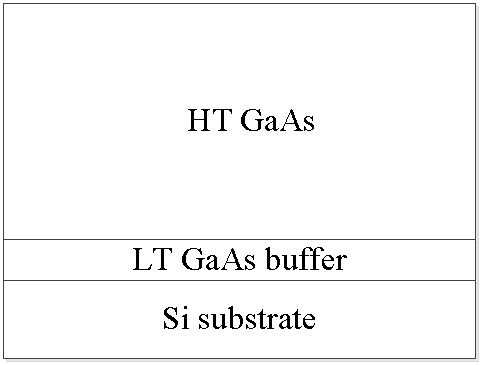
\includegraphics[width=0.8\textwidth]{ch03_TwoStepGrowth.pdf}
	\caption{TwoStep Growth}
	\label{fig:TwoStepGrowth}
\end{figure}

自从意识到用III族或V族元素钝化Si表面——在Si衬底上生长III-V族化合物的必要条件——导致了GaAs的最初生长是岛状生长,人们采取了许多不同的方法在Si衬底上沉积GaAs。包括:
使用外延衬底,例如先在Si衬底上沉积一层Si薄膜;低温生长最初的GaAs原子层;
用MEE外延方法分别外延Ga或As;生长无定形的Si或GaAs层。
到目前为止,应用最广泛的生长机制:两步法生长。
如图\ref{fig:TwoStepGrowth}所示,包括低温生长的GaAs缓冲层和最主要的高温生长的GaAs层。用这个生长顺序外延的原因是在结构位错产生之前低温生长的GaAs层是连续的。

\begin{figure}[ht]
	\centering
	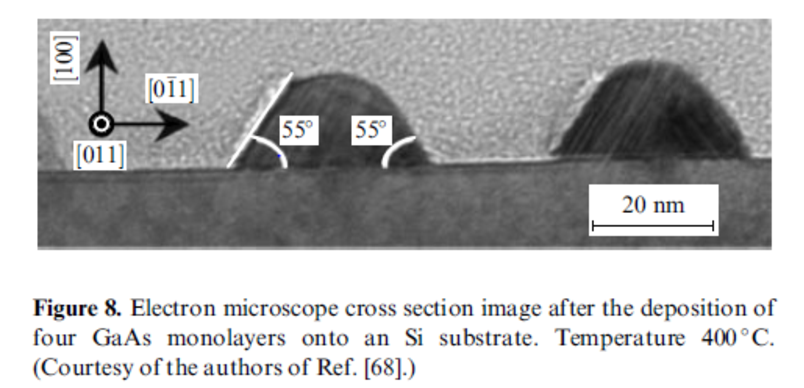
\includegraphics[width=0.8\textwidth]{ch03_GaAsIslands.pdf}
	\caption{GaAs Islands}
	\label{fig:GaAsIslands}
\end{figure}

在最初的生长阶段,GaAs岛的高度与横向宽度的比是1/2,而在Si衬底上生长的Ge的岛的高度与横向(\{105\}面)宽度的比是1/10。GaAs岛的高宽比远大于Ge岛,这表明Si基上GaAs成岛更加不可避免。图\ref{fig:GaAsIslands}是Si基上的GaAs岛的截面图。这些岛是在400℃的条件下沉积几个原子层的GaAs形成的,从图\ref{fig:GaAsIslands}中可以看出,这些岛是半球形的并且已经形成位错。

Si基上的GaAs岛可以看做是半球形,基于初期赝形生长的岛应力和形变计算,岛与衬底的界面是弯曲的,应力集中在岛的边缘,并且容易形成失配位错和其他的位错。
在1975年,Stowell详细地描述了在最初的薄膜沉积过程中,3D岛的合并导致了大量穿透位错的产生。
因此,人们需要研究在怎样的生长条件下失配位错能够产生在连续生长的薄膜中。


\begin{figure}[ht]
	\centering
	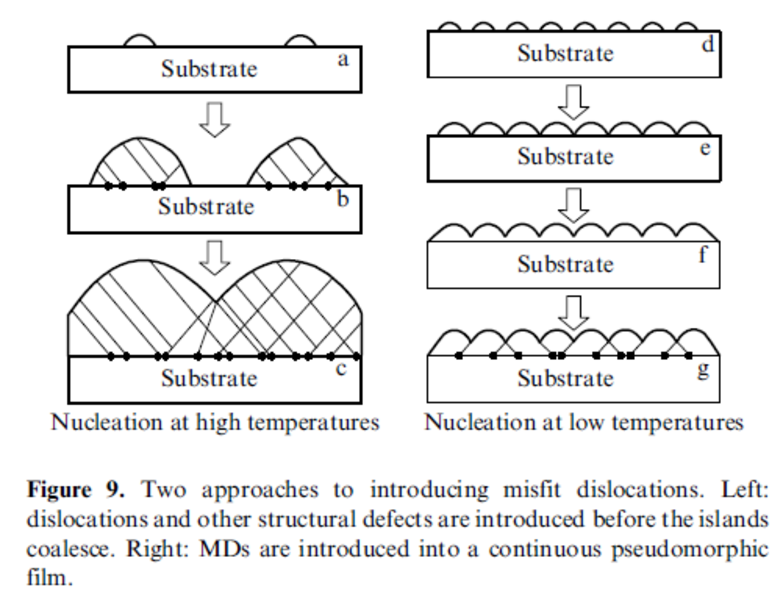
\includegraphics[width=0.8\textwidth]{ch03_IslandsGrowthProcedure.pdf}
	\caption{Islands Growth Procedure}
	\label{fig:IslandsGrowthProc}
\end{figure}

最初的生长温度越低,成岛的原子扩散区域越小,因此岛的密度就越大。图\ref{fig:IslandsGrowthProc}中是GaAs通过岛的合并形成层状的两种方式:一种是高温生长,另一种是低温生长。
以GaAs的生长温度为550℃-600℃为标准,当生长温度为400℃时,GaAs岛在合并之前就已经形成位错(图\ref{fig:IslandsGrowthProc}b),当这些岛开始合并时(图\ref{fig:IslandsGrowthProc}c),大量移动位错产生,这些位错用退火、高温生长厚外延层等方法都很难消除。

如果赝型生长的GaAs岛的合并方式如图 \ref{fig:IslandsGrowthProc}e和图\ref{fig:IslandsGrowthProc}f,粗糙的表面会产生很多位错,
这些位错会引入到连续生长的GaAs薄膜中(图\ref{fig:IslandsGrowthProc}g)。
因为低温生长的岛的密度比高温生长的岛的密度至少要高一个数量级,所以会导致表面形成的位错密度也较高(图\ref{fig:IslandsGrowthProc}f和图\ref{fig:IslandsGrowthProc}g)。
然而经实验表明,最初的GaAs薄膜用低温生长的GaAs外延层会降低XRD摇摆曲线的FWHM,表明提高了外延片的晶体质量。这应该怎么解释呢?一个可能的答案就是在GaAs合并时形成的失配位错变化较少,移动能力较强,所以在生长过程中,许多位错都能够消失。

据我们所知,到目前为止,对于初期的GaAs/Si的生长并没有详细的纳米级研究,因此不能直接观察到岛状生长到连续生长之间的变化。但是大量实验表明最初的GaAs用低温生长可以极大地改善GaAs外延层的晶体质量,但是这种生长方式的机制需要进一步的研究。


\section{衬底处理}

我们所使用的Si (001) 衬底是由天津通美公司提供的,偏角为偏向<011>4°。

对于Si衬底,表面常常有O,C杂质污染,在空气中极容易形成Si-O键,而作为外延薄膜衬底,它必须是完整,清洁并具有特定晶向,其中$SiO_x$可在超高真空下加热至1000℃把它除掉,但对于C污染,去除比较困难,表面上的SiC小团对外延层又非常有害,因此,必须寻找化学方法对Si表面进行处理。由于Si-O键的键能(439kJ/mol)比较大,而Si-H键的键能(222kJ/mol)比较小,因此Si表面极易被氧化,形成的氧化膜很稳定,要打开Si-O键所需的温度高于1000℃,而打开Si-H键所需的温度低于800℃。而MOCVD生长的温控平台一般为电热石墨舟结构,温度不宜长时间过高(>900℃)。如果不能在生长前断开所有的Si-O键去氧化,GaAs原子就很难与Si表面原子成键,导致外延质量急剧下降,因此Si片的氢化是非常重要的一步,另外Si表面一般还会吸附C等杂质,必须进行化学清洗。

1.首先预处理Si衬底,包括清洗、氢化、甩干。

第一步,用丙酮进行超声清洗,去除表面油脂等有机物。第二步,在$H_2 SO_4:H_2 O_2=3:1$溶液里煮洗至$H_2 O_2$完全挥发冒白烟,去除大部分有机物。第三步,在$NH_3•OH:H_2 O_2:H_2 O=1:1:6$溶液中,加热至75℃~85℃10min(由于氨水对硅有腐蚀作用,所以时间不能太长),去除金属杂质。第四步,在$HCl:H_2 O_2:H_2 O=1:1:6$,加热至75℃~85℃,盐酸对硅无腐蚀作用,可加热使得$H_2 O_2$完全挥发,去除表面金属离子。第五步,用HF漂洗5-10s,去除表面氧化层。第六步,用甩干机甩干并置入手套箱,尽量减少Si衬底与空气的接触时间。

2.高温烘烤、As钝化

经预处理的Si衬底送入反应室后,升温至750℃烘烤15min,烘烤的目的是使Si-H键脱离,然后在此温度下通入$AH_3$钝化3min,目的是使生长时先形成Si-As键,它相比Si-Ga更易成键。如前所述,这样可以减少反相畴和进一步清洁Si表面,以便为下一步生长做准备。
基于低温缓冲层的GaAs/Si直接外延的基本生长条件为:

\begin{enumerate}[(1)]
	\item 反应室压力为100Torr;
	\item 石墨舟转速为100rpm;
	\item III族源和V族源的载气(H2)总流量为12L/min;
	\item 三区石墨加热器的Zone A/B/C Ratio分别设定为39\%、45\%和80\%;
\end{enumerate}




\section{分项优化}

\subsection{低温缓冲层温度的优化}

大量实验表明,最优的低温缓冲层的生长温度在400-450℃之间,当第一步低温GaAs的生长温度高于450℃时,第二步高温GaAs的表面将变得粗糙;当第一步低温GaAs的生长温度低于400℃时,GaAs沉积可能不会发生。因此我们对低温缓冲层的温度进行了优化。

\begin{table*}[htbp] 
	\centering
	\caption{\label{tab:test1}低温缓冲层温度的优化}  
	\begin{tabular}{m{.15\textwidth}<{\centering}m{.3\textwidth}<{\centering}m{.25\textwidth}<{\centering}}   
		\toprule
			Sample no. & LT buffer growth temperature(℃) & DCXRD FWHM (arcsec) \\
		\midrule 
			A1 & 450 & 470.9 \\
			A2 & 460 & 501.3 \\
			A3 & 440 & 462.2 \\
			A4 & 420 & 462.6 \\
		\bottomrule
	\end{tabular}
\end{table*}

这一系列的样品低温缓冲层的温度分别为460、450、440和420℃,其他生长条件都是完全一样的:高温层的生长温度为630℃,生长速率为        ,生长厚度为900nm,且这些样品的表面都是光亮的。上图给出了不同低温缓冲层的生长温度对于外延片XRD半高宽的影响,可以看出当低温缓冲层的温度为440℃和420℃时,测得的XRD半高宽基本相同(462arcsec),我们选取了420℃作为了后续低温缓冲层的生长温度。

\begin {figure}
	\begin{minipage}[t]{0.33\linewidth}
		\centering
		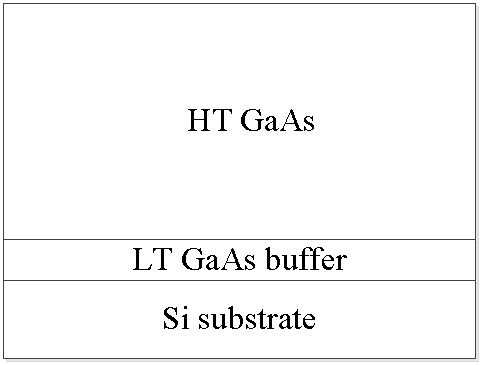
\includegraphics[width=1.2in]{ch03_TwoStepGrowth.pdf}
		\caption{fig1}
		\label{fig:side:a}
	\end{minipage}%
	\begin{minipage}[t]{0.33\linewidth}
		\centering
		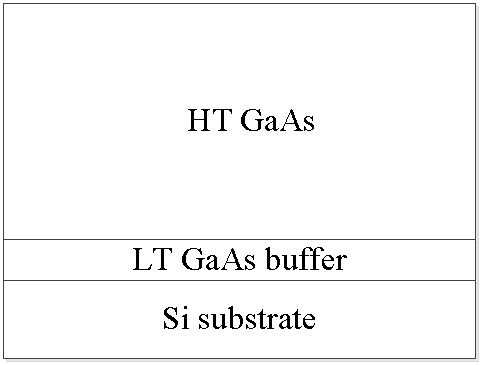
\includegraphics[width=1.2in]{ch03_TwoStepGrowth.pdf}
		\caption{fig2}
		\label{fig:side:b}
	\end{minipage}
	\begin{minipage}[t]{0.33\linewidth}
		\centering
		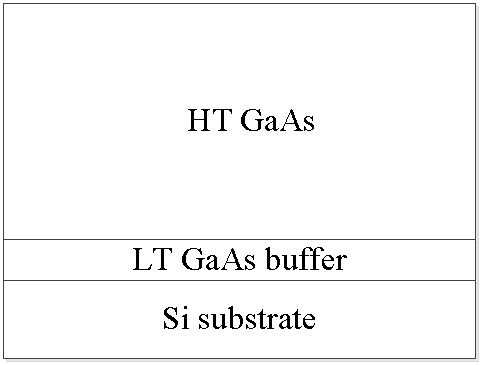
\includegraphics[width=1.2in]{ch03_TwoStepGrowth.pdf}
		\caption{fig2}
		\label{fig:side:b}
	\end{minipage}
\end{figure}



\begin{figure}
	\centering
	\subfigure[] {
		\label{fig:subfig:a} %% label for first subfigure 
		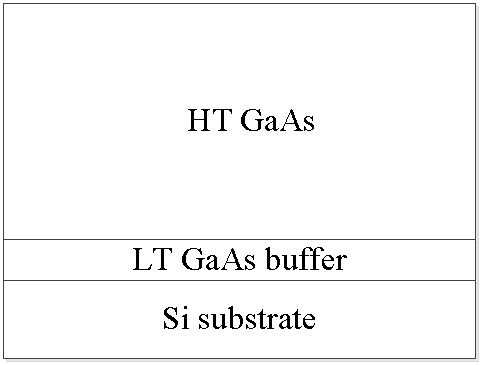
\includegraphics[width=1.5in]{ch03_TwoStepGrowth.pdf}
	} 
	\subfigure[] {
		\label{fig:subfig:b} %% label for second subfigure 
		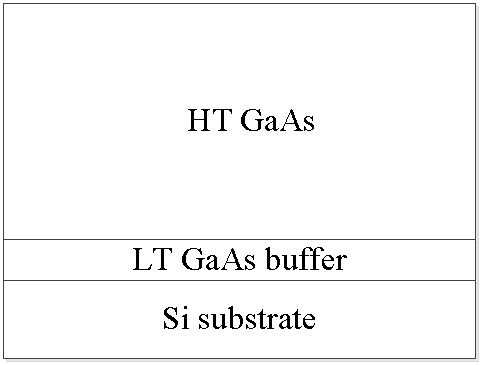
\includegraphics[width=1.5in]{ch03_TwoStepGrowth.pdf}
	} 
	\subfigure[] {
		\label{fig:subfig:b} %% label for second subfigure 
		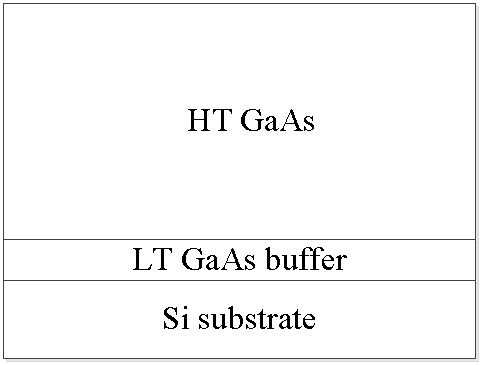
\includegraphics[width=1.5in]{ch03_TwoStepGrowth.pdf}
	} 
	\caption{Two Subfigures}
	\label{fig:subfig} %% label for entire figure
\end{figure}

\subsection{低温缓冲层厚度的优化}

\begin{table*}[htbp] 
	\centering
	\caption{\label{tab:test2}低温缓冲层厚度的优化}  
	\begin{tabular}{m{.1\textwidth}<{\centering}m{.3\textwidth}<{\centering}m{.2\textwidth}<{\centering}m{.25\textwidth}<{\centering}}   
		\toprule
			Sample no. & LT buffer growth time(s) & DCXRD FWHM (arcsec) & RMS roughness (nm) in 10μm×10μm \\
		\midrule
			A1 & 400 & 431.1 & 6.991 \\
			A2 & 600 & 412.9 & 3.641 \\
			A3 & 800 & 447.6 & 3.23 \\
		\bottomrule
	\end{tabular}
\end{table*}

当高温层生长温度和厚度固定(温度:685℃,厚度:900nm),低温缓冲层生长温度为420℃时,优化低温缓冲层的生长时间,即优化低温缓冲层的厚度。当低温缓冲层生长时间为600s(后经TEM测试,此时厚度为70nm)时,外延片的XRD半高宽最窄,晶体质量最好,所以选取低温缓冲层厚度70nm作为后续外延片生长的低温缓冲层厚度。


\subsection{低温缓冲层种类的优化}

仅仅依靠高温生长并不能满足整个异质结构对于GaAs/Si外延片的要求,当最初的生长层的厚度、掺杂浓度和掺杂类型不同的时候,接下来的生长温度就不能超过一个固定的限制。由于这个原因,人们在GaAs和Si衬底之间采用不同材料的低温缓冲层,

\begin{table*}[htbp] 
	\centering
	\caption{\label{tab:test3}低温缓冲层种类的优化}  
	\begin{tabular}{m{.1\textwidth}<{\centering}m{.3\textwidth}<{\centering}m{.2\textwidth}<{\centering}m{.25\textwidth}<{\centering}}   
		\toprule
			Sample no. & Growth procedure & DCXRD FWHM (arcsec) & RMS roughness (nm) in 10μm×10μm \\
		\midrule
			A1 & GaAs buffer layer & 412 & 3.6 \\
			A2 & AlAs buffer layer & 401 & 3.4 \\
			A3 & AlGaAs/GaAs buffer layer & 447 & 6.3 \\
		\bottomrule
	\end{tabular}
\end{table*}

在固定的低温缓冲层生长温度和厚度(温度:420℃,厚度:70nm)、固定的高温层生长温度和厚度(温度:685℃,厚度:900nm)下,当低温缓冲层为AlAs时,XRD半高宽最窄,晶体质量最好。但是由于Al易氧化,后续的生长没有采用AlAs缓冲层。

\section{结论}

我来占个位置。\cite{BUPT_Thesis_Format_2004}

% 本章参考文献
\ifx\usechapbib\empty
\bibliographystyle{buptthesis}
\bibliography{bare_thesis}
\fi

%%% Local Variables: 
%%% mode: latex
%%% TeX-master: "bare_thesis"
%%% End: 
